%This work is licensed under the Creative Commons License Attribution 4.0 International (CC-BY 4.0)
%https://creativecommons.org/licenses/by/4.0/legalcode
\documentclass[rgb]{standalone}
\usepackage{tkz-euclide}
\definecolor{myorange}{hsb}{0.0833, 1, 0.8}
\definecolor{mygreen}{hsb}{0.3333, 1, 0.8}
\definecolor{myblue}{hsb}{0.5833, 1, 0.8}
\definecolor{mymagenta}{hsb}{0.8333, 1, 0.8}
\begin{document}
	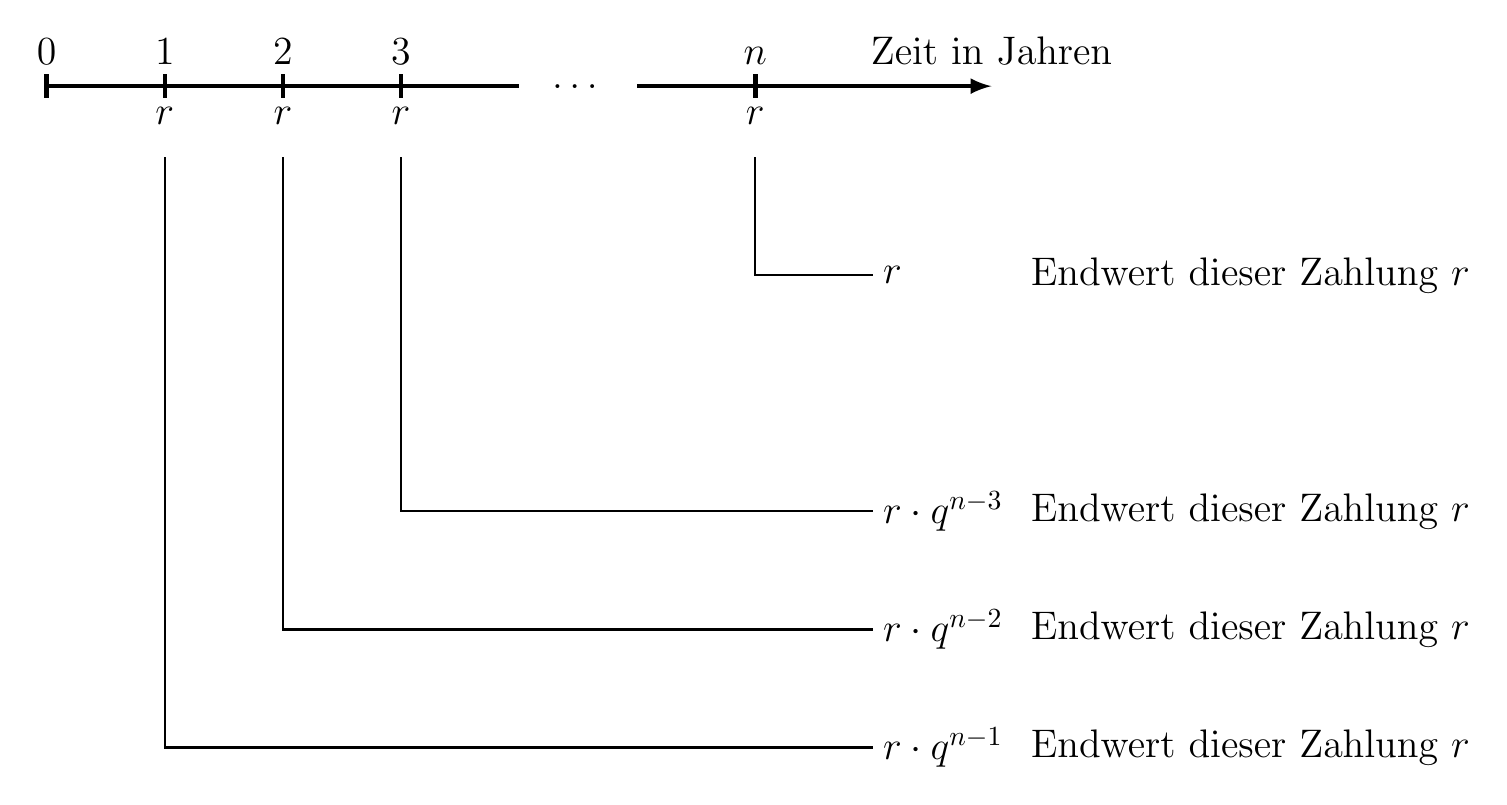
\begin{tikzpicture}[scale=1.5, font=\Large]
        \draw[ultra thick] (0,0) -- (4,0);
        \draw[ultra thick,-latex] (5,0) -- (8,0);
        \draw[ultra thick] (0,-0.1) -- (0,0.1);
        \draw[ultra thick] (1,-0.1) -- (1,0.1);
        \draw[ultra thick] (2,-0.1) -- (2,0.1);
        \draw[ultra thick] (3,-0.1) -- (3,0.1);
        \draw[ultra thick] (6,-0.1) -- (6,0.1);
        \draw[thick] (6,-0.6) -- (6,-1.6) -- (7,-1.6);
        \draw[thick] (3,-0.6) -- (3,-3.6) -- (7,-3.6);
        \draw[thick] (2,-0.6) -- (2,-4.6) -- (7,-4.6);
        \draw[thick] (1,-0.6) -- (1,-5.6) -- (7,-5.6);
        \node[above] at (0,0.1) {$0$};
        \node[above] at (1,0.1) {$1$};
        \node[above] at (2,0.1) {$2$};
        \node[above] at (3,0.1) {$3$};
        \node[above] at (6,0.1) {$n$};
        \node[above] at (8,0.1) {Zeit in Jahren};
        \node[below] at (1,-0.1) {$r$};
        \node[below] at (2,-0.1) {$r$};
        \node[below] at (3,-0.1) {$r$};
        \node[below] at (6,-0.1) {$r$};
        \node[right] at (7,-1.6) {$r$};
        \node[right] at (7,-3.6) {$r\cdot q^{n-3}$};
        \node[right] at (7,-4.6) {$r\cdot q^{n-2}$};
        \node[right] at (7,-5.6) {$r\cdot q^{n-1}$};
        \node[right] at (8.25,-1.6) {Endwert dieser Zahlung $r$};
        \node[right] at (8.25,-3.6) {Endwert dieser Zahlung $r$};
        \node[right] at (8.25,-4.6) {Endwert dieser Zahlung $r$};
        \node[right] at (8.25,-5.6) {Endwert dieser Zahlung $r$};
        \node[anchor=center] at (4.5,0) {\ldots};
%\draw[-,line width=2pt] (0,0)--(4,0);
%\draw[-,line width=2pt] (0,-0.25)--(0,0.25);
%\node[above] at(0,0.25){$0$};
%\draw[-,line width=2pt] (1,-0.25)--(1,0.25);
%\node[below] at(1,-0.25){$r$};
%\node[above] at(1,0.25){$1$};
%\draw[-,line width=2pt] (1,-1)--(1,-6);
%\draw[-,line width=2pt] (1,-6)--(7,-6);
%\node[right] at(7,-6){$r \cdot q^{n-1}$\ \ Endwert dieser Zahlung $r$};
%\draw[-,line width=2pt] (2,-0.25)--(2,0.25);
%\node[below] at(2,-0.25){$r$};
%\node[above] at(2,0.25){$2$};
%\draw[-,line width=2pt] (2,-1)--(2,-5);
%\draw[-,line width=2pt] (2,-5)--(7,-5);
%\node[right] at(7,-5){$r \cdot q^{n-2}$\ \ Endwert dieser Zahlung $r$};
%\draw[-,line width=2pt] (3,-0.25)--(3,0.25);
%\node[below] at(3,-0.25){$r$};
%\node[above] at(3,0.25){$3$};
%\draw[-,line width=2pt] (3,-1)--(3,-4);
%\draw[-,line width=2pt] (3,-4)--(7,-4);
%\node[right] at(7,-4){$r \cdot q^{n-3}$\ \ Endwert dieser Zahlung $r$};
%\node at(4.5,0){...};
%\draw[->,line width=2pt] (5,0)--(8,0);
%\draw[-,line width=2pt] (6,-0.25)--(6,0.25);
%\node[below] at(6,-0.25){$r$};
%\node[above] at(6,0.25){$n$};
%\draw[-,line width=2pt] (6,-1)--(6,-2);
%\draw[-,line width=2pt] (6,-2)--(7,-2);
%\node[right] at(7,-2){$r$\ \ \ \ \ \ \ \ \ \ \ \ Endwert dieser Zahlung $r$};
%\node[above] at(8,0.25){Zeit in Jahren};
  \end{tikzpicture}
\end{document}